\chapter{Review of Strain Estimation Techniques}

Imaging strain is one fundamental application of OCE, which produces qualitative images of the stiffness of tissue. The tissue strain is defined as the amount of displacement induced in the tissue by the mechanical loading per spatial region. It is calculated by estimating the spatial derivative of the displacement imaged by the OCE system. Making the assumption that tissue is a linearly elastic solid, the displacement can be thought of as linearly related to the depth into the sample. Under small enough compressions this assumption is valid. 

To be able to compare between imaging techniques, the resolution of different strain estimation fits must be derived. This resolution can be thought of as the full-width at half maximum of the impulse response of the filter - that is, the FWHM of the output when the input signal is a delta function in the case of a smoothing filter, or a step function for the differentiation filters. This resolution offers a comparative measure of the extent to which the filtering process has blurred objects in the image together. 

\section{Least Squares Approaches}
Least squares approach aim to fit a straight line to the phase data by minimising the squared error between the fitted and actual values. The strain value is then taken to be the gradient of this line. The ordinary least squares estimate for the strain value within a fit window of size $m$ is given in \cite{kennedy_strain_2012} as:

\begin{equation}
	\label{ols_strain}
	\epsilon_z = \sum\limits_{j=1}^{j=i+m-1} \bigg(\frac{\kappa_0 (z_j-z_{i-1})-\kappa_1}{\kappa_0 \kappa_2 - \kappa_1^2} \bigg) u_j
\end{equation}

Where $u_j$ is the displacement at the point, and the simplifying constants $\kappa_x$ are defined as:

\begin{equation}
	\label{ols_k}
	\kappa_x = \sum \limits_{j=1}^{i+m-1} (z_j - z_{i-1})^x \text{   for   } x = 0,1,2
\end{equation}

Depending on the size of the fit window, there is a likelihood of a wrapping event to have occurred, and therefore there is a need to unwrap the phase (displacement) data prior to performing a least squares estimate. 

The ordinary least squares estimate above is a linear operation, however can be extended to use weight the contribution of each displacement point based on the quality of its signal. The weighted least squares strain estimate utilises the OCT signal attached to each phase difference value to provide an estimate of the standard deviation of each point. The variance of the measured phase difference is equal to the inverse of the SNR of the OCT intensity, $SNR_{OCT}$. Therefore a $\Delta \phi_i$ measurement that has a high $SNR_{OCT}$ has a low variance, and should be assigned more significance in estimating a linear displacement fit. Therefore the weights associated with the weighted least squares estimate is the inverse variance of the phase difference values:

\begin{equation}
	\label{wls_w}
	w_i = \frac{1}{\sigma_{u_j}^2} = SNR_{OCT_j}
\end{equation}

Using these weights, the strain estimate using weighted least squares is given as in \cite{kennedy_strain_2012} by Equation \ref{wls_strain}:

\begin{equation}
	\label{wls_strain}
	\epsilon_i = \sum \limits_{j=1}^{i+m-1} \frac{\kappa'_0 w_j (z_j - z_{i-1}) u_j - \kappa'_1 w_	j u_j}{\kappa'_0 \kappa'_2 - (\kappa'_1)^2}
\end{equation}

Where in this instance, the $\kappa'_x$ constants are given by:

\begin{equation}
	\label{wls_k}
	\kappa'_x = \sum \limits_{j=1}^{i+m-1} w_j (z_j - z_{i-1})^x \text{   for   } x=0,1,2
\end{equation}

The weighted least squares strain estimate has been shown to improve the strain sensitivity \cite{kennedy_strain_2012} however at the expense of requiring the calculation of the weightings, and the non-linearity of the operation, the consequences of which are discussed in the next section.

\section{Savitzky-Golay Filtering}
One benefit of the ordinary least squares approach is that it can be implemented as a filter, since it is a linear operation. The Savitzky-Golay filter \cite{savitzky_smoothing_1964} can be applied to data to smooth it to a linear fit, equivalent to performing a least squares estimate. This filter can be applied to an entire data set by convolving the data and filter together, or a multiplying them in the Fourier domain. Similarly to how the estimate above for ordinary least squares is derived using the normal equation for least squares minimization (see Appendix 1), the Savitzky-Golay filter is derived by assuming the data is centred around zero and scaled in integer steps, and calculating the filter coefficients for these points for the given fitting model (in this case, linear), and then generalising them to all fit windows. A more detailed derivation can be found in \cite{savitzky_smoothing_1964}. The Savitzky-Golay smoothing filter based on the least squares approximation can be generalised to a Savitzky-Golay differentiation filter by evaluating the gradient, rather than the value, at each point. There is an analytical solution for the Savitzky-Golay first order differentiation filter for a linear least squares model given in Equation \ref{sg_coeff} \cite{madden_comments_1978}.

\begin{equation}
	\label{sg_coeff}
	C_i = \frac{12 i}{m(m^2-1)}
\end{equation}

Therefore not only can the filter be applied much faster than a sequential looping over the fit windows and performing the ordinary least squares estimate above, it can be created very quickly as well. However, the weighting information can no longer be utilised in the convolution process. Another aspect to note, is that the Savitzky-Golay filter can only be applied on the unwrapped phase difference - it cannot correct for wrapping events. 

The resolution of the Savitzky-Golay filter can be derived by analysing it's response to an impulse. It can be seen that the impulse response of the filter is quadratic in form, and the FWHM can be solved for, giving the value in Equation \ref{sg_fwhm}:

\begin{equation}
	\label{sg_fwhm}
	\text{FWHM}_{SG} = \frac{m}{\sqrt{2}}
\end{equation}

\section{Smoothing Filters}
In most biological signal processing, high frequency noise is a significant degrading factor, one that is amplified in applications such as elastograpy where derivatives are estimated to produce the signal \cite{usui_digital_1982}. As a result, low-pass differentiation filters are ideal signal processing techniques. The Savitzky-Golay filter acts as a low-pass differentiation filter \cite{luo_axial_2004}, as does a sequential application of weighted least squares. However the simple finite difference strain estimation described in Section 3.1 makes no effort to smooth out high frequency noise. It makes sense to combine a low-pass smoothing filter with the finite difference derivative estimation in order to do this. Since linear filter operations are commutative, the filter convolution operation can be done to the phase difference or to the finite difference strain estimate. This smoothing filter could be implemented as a simple moving average, however with the goal of minimising the contribution of high frequency noise, it makes sense to take a Gaussian smoothing filter, the discretised version of which is seen in Equation \ref{gauss_1d} for a 1D filter, and \ref{gauss_2d} for the 2D filter.

\begin{equation}
	\label{gauss_1d}
	G^{1D}_i = \frac{1}{\sqrt{2\pi} \sigma} \exp{\bigg(\frac{-(i_0-i)^2}{2 \sigma^2}\bigg)}
\end{equation}

\begin{equation}
	\label{gauss_2d}
	G^{2D}_{ij} = \frac{1}{2\pi \sigma_i \sigma_j } \exp{ 
	\bigg( - \frac{(i_0 - i)^2}{2 \sigma_i^2} - \frac{(j_0 - j)^2}{2 \sigma_j^2} \bigg)}
\end{equation}

Using a Gaussian smoothing filter in addition to finite difference removes high frequency noise, where the resolution of this smoothing filter is defined as the FWHM of the Gaussian filter used, dependent on the $\sigma$ value as shown in Equation \ref{gauss_fwhm}.

\begin{equation}
	\label{gauss_fwhm}
	\text{FWHM}_{Gaussian} = 2 \sqrt{2 \log{2}} \sigma
\end{equation}

\section{Finite Difference}
The simplest approximation to a derivative is to calculate the finite difference between two consecutive displacement measurements. That is, dividing the change in displacement by the change in depth, as per Equation \ref{fd_strain}.

\begin{equation}
	\label{fd_strain}
	\epsilon_z = \frac{\Delta u_z}{\Delta z}
\end{equation}

An issue with finite difference approaches is that they tend to amplify high frequency noise in the phase values. However one of its benefits is the simplicity of implementation, and therefore the speed up it offers. In addition, by using consecutive pixels to perform the differentiation, there is little chance of a phase wrapping event to have occurred, and therefore finite difference can be performed on the complex phase data without prior unwrapping.

Since there is no smoothing operation implemented in finite difference, it is assumed that it has no effect on the resolution of the image. Therefore there is no assumed a negligible fit resolution contribution using the finite difference strain estimation, and the fit resolution is instead defined by smoothing operations that are implemented alongside it.

\section{Strain Estimation Assessment Criteria}

\subsection{Sensitivity}
The strain sensitivity is defined as the minimum detectable strain in the elastogram \cite{kennedy_strain_2012}, a quantity that gives insight into how well the OCE imaging system and signal processing is capable of reproducing the physical displacement and strain in the imaged sample. If the strain sensitivity is too large, then it is not possible to detect differences between stiff and soft objects (such as stroma and tumour) without having a much larger compressive force, which invalids many assumptions previously made (such as the linear elasticity of tissue, and uniaxial compression). Therefore it is important to use the strain sensitivity as a metric of image quality. 

The strain sensitivity is defined as the standard deviation of the strain values within a region of uniform elasticity \cite{varghese_theoretical_1997}, such as can be artificially created using a phantom. The ideal characteristics of the region include absence of artefacts, including those that occur near the sample surface reflection, and at a depth shallow enough to minimise the attenuation of the OCT signal and decorrelation noise. Such a region is shown in Figure \ref{sensitivity_region} for a silicon phantom with a stiff inclusion. 

\subsection{Image Resolution}
The image resolution can be thought of as the ability to distinguish between two objects in the resulting strain elastogram. Traditionally, this has been examined in terms of the impulse response of an optical system, more directly as the FWHM of this impulse response \cite{reynolds_resolution_1989}. However we typically don't have access to the impulse response of the combined strain estimation filter and optical system response, therefore another method of quantifying the image resolution is used based on a previous Masters project \cite{hepburn_improving_2017}.

\begin{figure}[t]
	\centering
	\begin{subfigure}{0.49\textwidth}
		\centering
		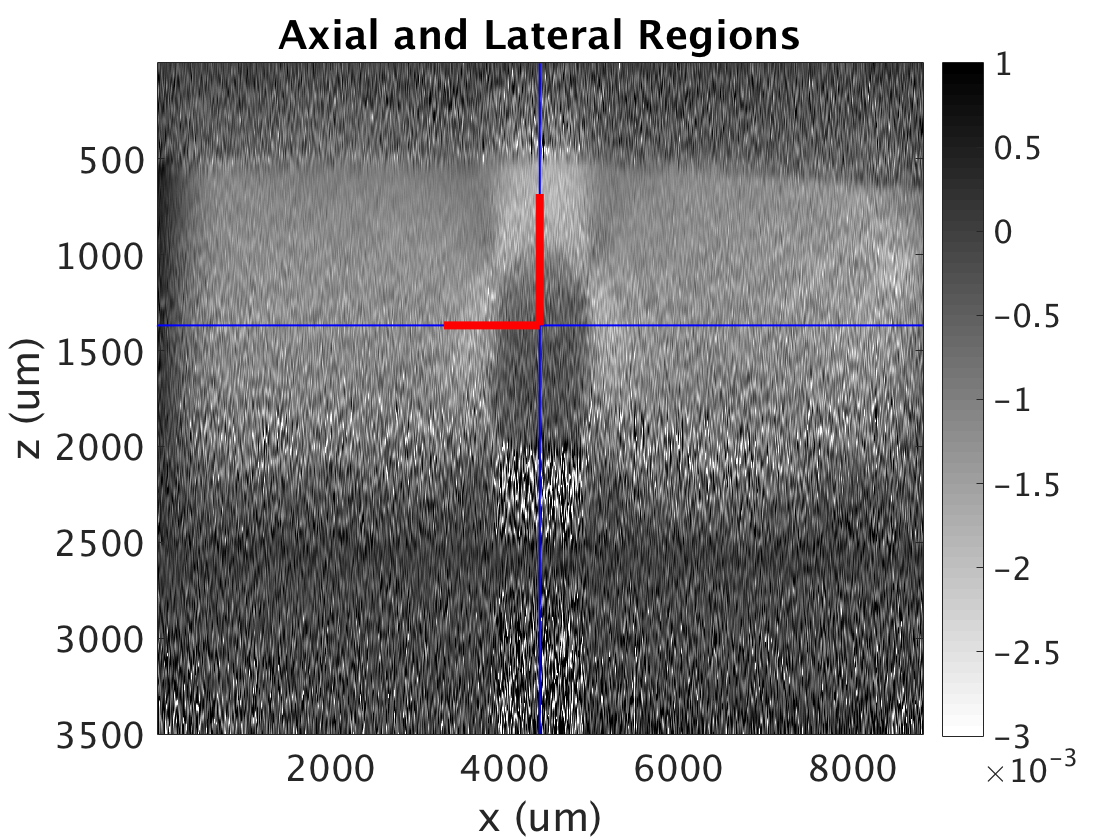
\includegraphics[width=\textwidth]{figures/image_res_regions.png}
	\end{subfigure}
	\begin{subfigure}{0.49\textwidth}
		\centering
		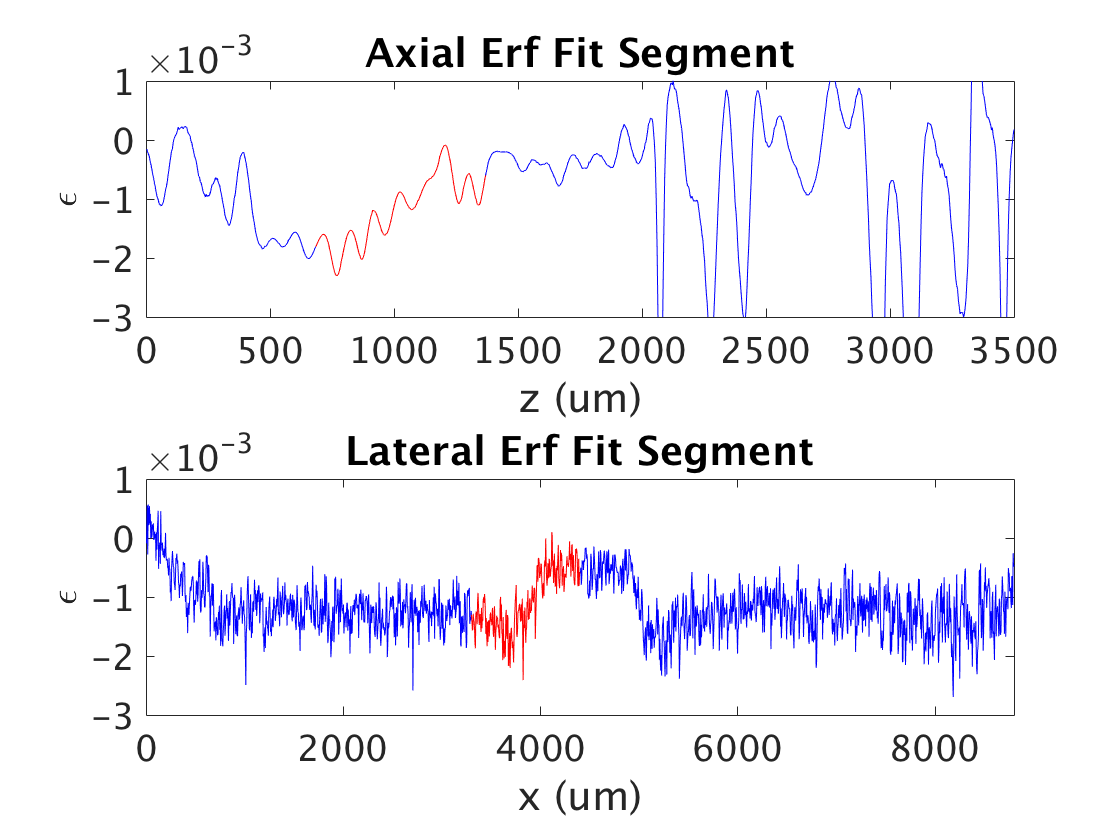
\includegraphics[width=\textwidth]{figures/lateral_axial_segments.png}
	\end{subfigure}
	\label{axial_lateral_regions}
	\caption{The segments used to calculate the image resolution for both axial and lateral directions, shown imposed on the strain elastogram in a) where the blue corresponds to the scan taken, and the red the region the error function is fitted over. Part b) shows the plots of these scans and segments, with the axial above, and lateral below.}
\end{figure}

The image resolution is thought of as the 'speed' of transition from one uniform strain region to another, as measurable in a phantom sample which has clearly defined regions of different stiffness. This transition can be seen in both the axial and lateral directions, as shown in Figure \ref{axial_lateral_regions}.

\begin{figure}[t]
	\centering
	\begin{subfigure}{0.49\textwidth}
		\centering
		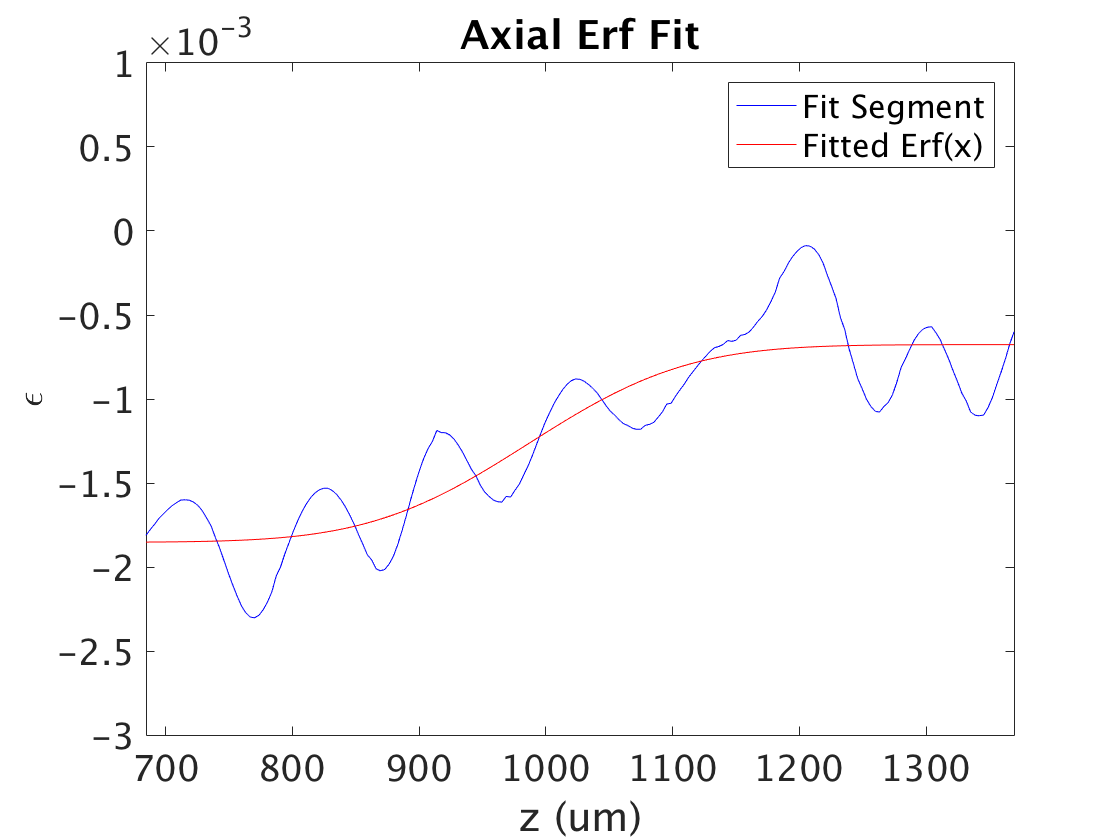
\includegraphics[width=\textwidth]{figures/axial_erf_fit.png}
	\end{subfigure}
	\begin{subfigure}{0.49\textwidth}
		\centering
		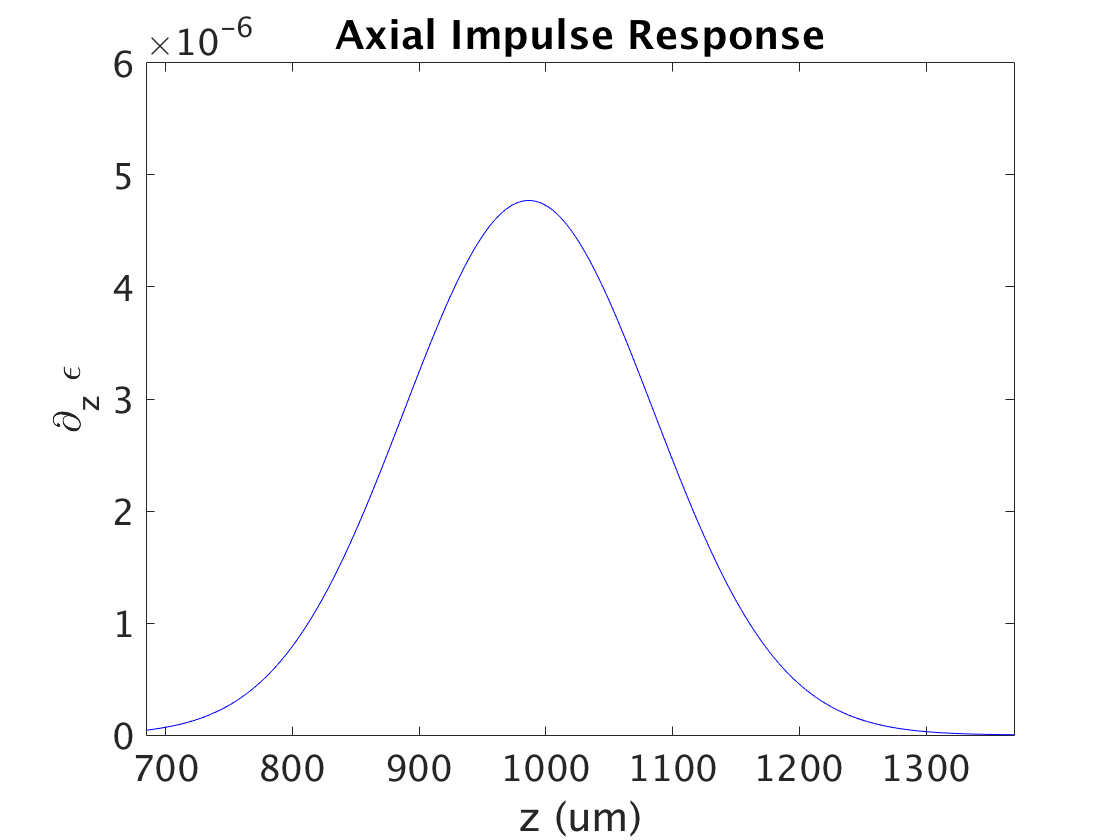
\includegraphics[width=\textwidth]{figures/axial_impulse_response.png}
	\end{subfigure}
	\\
	\begin{subfigure}{0.49\textwidth}
		\centering
		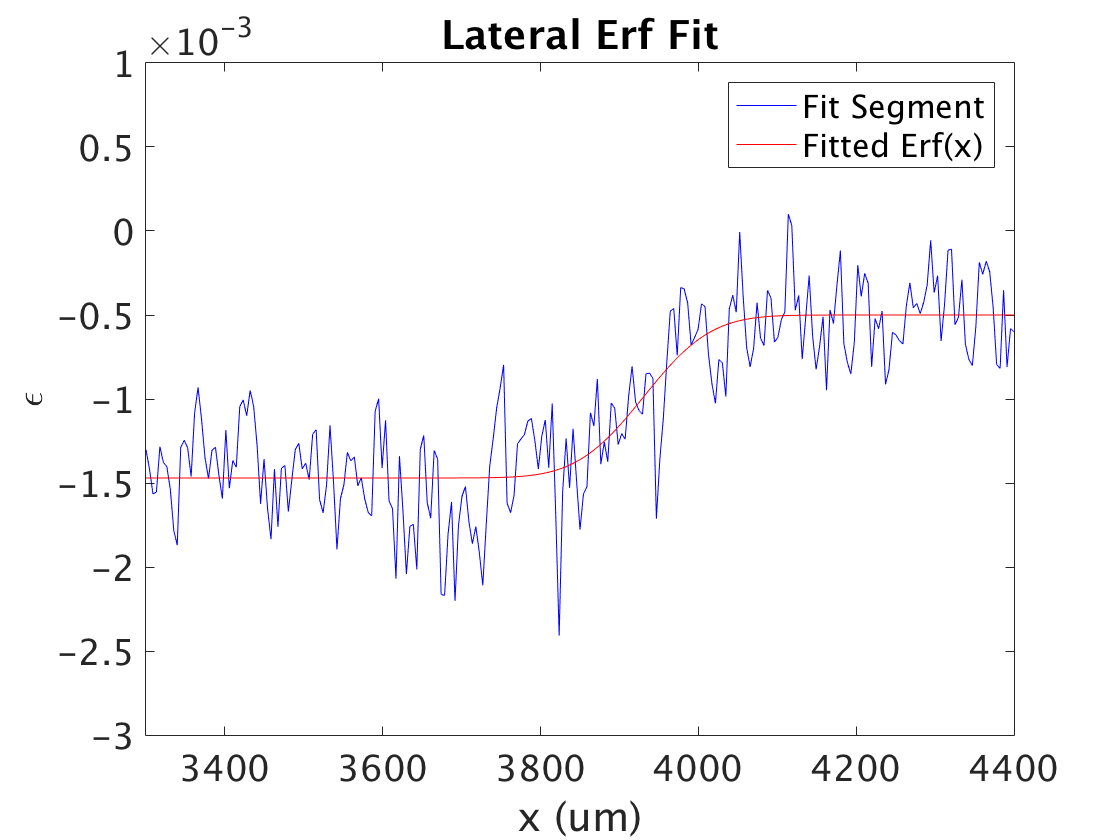
\includegraphics[width=\textwidth]{figures/lateral_erf_fit.png}
	\end{subfigure}
	\begin{subfigure}{0.49\textwidth}
		\centering
		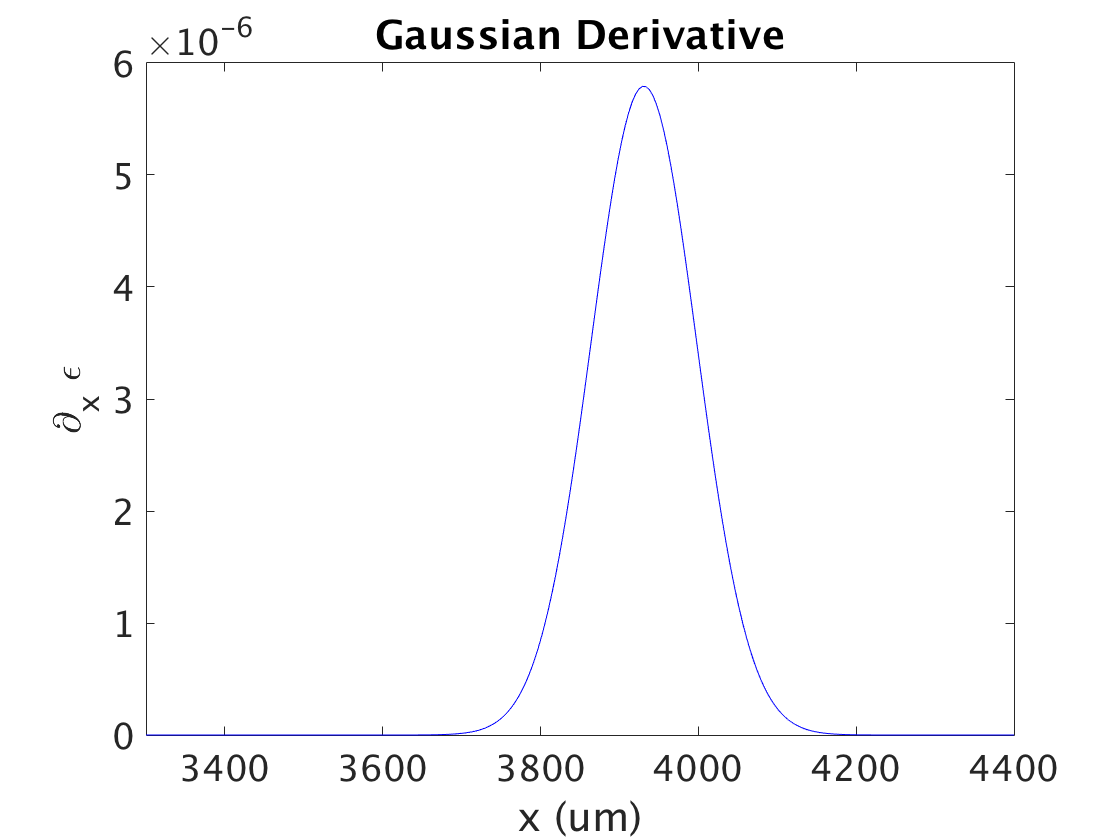
\includegraphics[width=\textwidth]{figures/lateral_impulse_response.png}
	\end{subfigure}
	\label{error_fit_example}
	\caption{The left images show the segment over the axial and lateral boundaries respectively with the overlaid error function fit. The right images show the impulse response, which is the derivative of the error function, for the fit, of which the FWHM is the image resolution.}
\end{figure}

The transition across a feature boundary in the strain elastogram can be approximated by an error function, as given in Equation \ref{erf_normal}, and visualised in Figure \ref{error_fit_example}. 

\begin{equation}
	\text{erf}(x)=\frac{1}{\sqrt{\pi}} \int_{-x}^{x} \text{e}^{-t^2}
	\label{erf_normal}
\end{equation}

The standard error function above can be translated and scaled (see Equation \ref{erf_scaled}) to allow fitting to the strain values over the boundary, and also to allow for the introduction of the parameter $a$ that governs the rise time of the error function. When this scaled error function is fitted to the strain data across the boundary, the $a$ parameter is the most significant and is used to calculate an image resolution.

\begin{equation}
	n \: \text{erf}(\:a(x-b)\:) + c = \frac{n}{\sqrt{\pi}} \int_{-(x-b)}^{(x-b)} \text{e}^{-a t^2} + c
	\label{erf_scaled}
\end{equation}

Once this analytical model is derived from the strain data, the derivative of the fitted error function provides the impulse response of the system, and it is the FWHM of this derivative that provides the image resolution \cite{hepburn_improving_2017}. For the scaled error function, the derivative is a similarly scaled Gaussian function, given in Equation \ref{gaussian_derivative}.

\begin{equation}
	G(x) = \frac{2\:a\:n}{\sqrt{\pi}} \text{e}^{-a^2 (x-b)^2}
	\label{gaussian_derivative}
\end{equation}

The FWHM of this Gaussian is given in Equation \ref{image_res_fwhm} and provides the image resolution in the direction specified (axial or lateral, as in Figure \ref{axial_lateral_regions}).

\begin{equation}
	\text{FWHM}_{IR} = \frac{2 \sqrt{\text{ln}(2)}}{a}
	\label{image_res_fwhm}
\end{equation}

\subsection{Processing Speed}
The processing speed of the strain estimation technique is not a standard metric for assessing the strain elastogram quality, but keeping in mind the motivation for this project it is of utmost importance.
The processing speed of the different strain estimation algorithms was assessed using both the processing of a single B-scan, and for a complete 3D volume. In addition, differences in algorithm complexity are pointed out between the methods, as well as the ease with which they can be parallelised, and the likelihood of a speed up made possible by parallelising the processing.

